%% 
%% Copyright 2007, 2008, 2009 Elsevier Ltd
%% 
%% This file is part of the 'Elsarticle Bundle'.
%% ---------------------------------------------
%% 
%% It may be distributed under the conditions of the LaTeX Project Public
%% License, either version 1.2 of this license or (at your option) any
%% later version.  The latest version of this license is in
%%    http://www.latex-project.org/lppl.txt
%% and version 1.2 or later is part of all distributions of LaTeX
%% version 1999/12/01 or later.
%% 
%% The list of all files belonging to the 'Elsarticle Bundle' is
%% given in the file `manifest.txt'.
%% 

%% Template article for Elsevier's document class `elsarticle'
%% with numbered style bibliographic references
%% SP 2008/03/01

\documentclass[preprint,12pt]{elsarticle}

%% Use the option review to obtain double line spacing
%% \documentclass[authoryear,preprint,review,12pt]{elsarticle}

%% Use the options 1p,twocolumn; 3p; 3p,twocolumn; 5p; or 5p,twocolumn
%% for a journal layout:
%% \documentclass[final,1p,times]{elsarticle}
%% \documentclass[final,1p,times,twocolumn]{elsarticle}
%% \documentclass[final,3p,times]{elsarticle}
%% \documentclass[final,3p,times,twocolumn]{elsarticle}
%% \documentclass[final,5p,times]{elsarticle}
%% \documentclass[final,5p,times,twocolumn]{elsarticle}

%% For including figures, graphicx.sty has been loaded in
%% elsarticle.cls. If you prefer to use the old commands
%% please give \usepackage{epsfig}

%% The amssymb package provides various useful mathematical symbols
\usepackage{amssymb}
%% The amsthm package provides extended theorem environments
%% \usepackage{amsthm}

%% The lineno packages adds line numbers. Start line numbering with
%% \begin{linenumbers}, end it with \end{linenumbers}. Or switch it on
%% for the whole article with \linenumbers.
\usepackage{lineno}
\usepackage{algorithm}
\usepackage{algorithmic}
\usepackage{graphicx}
\usepackage{subcaption}

\def\bibsection{\section*{References}}

\journal{Future Generation Computer Systems}

\begin{document}

\begin{frontmatter}

%% Title, authors and addresses

%% use the tnoteref command within \title for footnotes;
%% use the tnotetext command for theassociated footnote;
%% use the fnref command within \author or \address for footnotes;
%% use the fntext command for theassociated footnote;
%% use the corref command within \author for corresponding author footnotes;
%% use the cortext command for theassociated footnote;
%% use the ead command for the email address,
%% and the form \ead[url] for the home page:
%% \title{Title\tnoteref{label1}}
%% \tnotetext[label1]{}
%% \author{Name\corref{cor1}\fnref{label2}}
%% \ead{email address}
%% \ead[url]{home page}
%% \fntext[label2]{}
%% \cortext[cor1]{}
%% \address{Address\fnref{label3}}
%% \fntext[label3]{}

\title{ParSA: High-throughput Scientific-data Analysis Framework with Distributed File System}


%% use optional labels to link authors explicitly to addresses:
%% \author[label1,label2]{}
%% \address[label1]{}
%% \address[label2]{}

%\author{Tao Zhang}
%\ead{t-zhang11@mails.tsinghua.edu.cn}
%\address{Tsinghua}
\author[1]{Tao Zhang\corref{cor1}}
\ead{t-zhang11@mails.tsinghua.edu.cn}
\author[2]{XiangZheng Sun}
%\ead{xiangzheng.sun@intel.com}
\author[1]{Wei Xue}
%\ead{xuewei@mail.tsinghua.edu.cn}
\cortext[cor1]{Corresponding author. Tel: +86 18210192568}
\address[1]{Department of Computer Science and Technology, Tsinghua University, Beijing, China}
\address[2]{Intel Corporation, Beijing, China}

\begin{abstract}
Scientific-data analysis and visualization has become a key component in nowadays large-scale simulations. Due to the rapidly
increasing data volume and awkward I/O pattern among high-structured files, known serial methods/tools cannot scale well and 
usually lead to poor performance over traditional architectures. In this paper, we propose a new framework: ParSA 
(parallel scientific-data analysis) for high-throughput and scalable scientific analysis, with distributed file system. ParSA
presents the optimization strategies for grouping and spliting logical units to maximize distributed I/O property of distributed 
file system as well as to maximize overlapping the data reading, processing and transferring during computation. Besides, ParSA 
provides the similar interfaces as the NCO (NetCDF Operator), which is used in most of climate data diagnostic packages, making
it easy to port this framework. We utilize ParSA to accelerate well-known analysis methods for climate models on Hadoop Distributed File 
System (HDFS). Experimental results demonstrate the high efficiency and scalability of ParSA, getting the maximum 1.2GB/s throughput.
\end{abstract}

\begin{keyword}
%% keywords here, in the form: keyword \sep keyword

%% PACS codes here, in the form: \PACS code \sep code

%% MSC codes here, in the form: \MSC code \sep code
%% or \MSC[2008] code \sep code (2000 is the default)
Data intensive \sep Scientific data analysis \sep Distributed file system
\end{keyword}

\end{frontmatter}

\linenumbers

%% main text
\section{Introduction}
In most of modern scientific applications, huge amounts of data are produced. Large-scale simulations, such as climate modeling,
high-energy physics simulation and genome mapping, generate hundreds of terabytes data volumes\cite{kosar2009new}\cite{hey2003data}. 
Additionally, it still increases as the high resolution model developping. As a consequence, analysis of scientific-data is 
data-intensive.\par
In fact, almost all of scientific-data are stored in high-structured files, some of which provide parallel I/O interface, such as
Network Common Data Format version 4 (NetCDF4)\cite{rew2006netcdf}, Hierarchical Data Format 5(HDF5)\cite{folk1999hdf5} and ADIOS BP data
format (BP) \cite{lofstead2008input}, and some of which only support serial I/O interface,  like Network Common Data Format version 3
(NetCDF3) \cite{rew1990netcdf}. All of them are self-describing, machine-independent data format. \par
In scientific-data analysis, large-scale scientific-data are stored in RAID-5/6 or parallel file system. Yet the analysis methods/
tools are always centralized approaches, such as NCO\cite{zender2008analysis} and NCL\cite{ncl}, which are the most used in climate 
applications for prossing NetCDF files, leading to very poor scalability and time-consuming performance. \par    
Inspired by big data solution in Internet Port Data Center (IPDC), numerous frameworks with distributed strategy have been developed.
MapReduce is a program framework for processing and generating large data sets, provideing automatic parallel mechanism and build-in 
fault-tolerance on a cluster\cite{dean2008mapreduce}. However, this solution with MapReduce requires data firstly to be transformed into 
a text-based format\cite{zhao2010parallel}. SciHadoop\cite{buck2011scihadoop} is a Hadoop plugin allowing scientists to specify logical 
queries over array-based data models. It executes queries as map/reduce programs defined over the logical data model. It shows remarkable 
improvements for holistic functions of NetCDF data sets for the following optimization goals: reduce total data transfers, reduce remote 
reads and reduce unnecessary reads. Nevertheless, SciHadoop using java language leads to the compatibility problem to the existing climate 
data analysis tools, which is written by C shell scripts, NCL and NCO commands. The SWAMP project \cite{wang2008clustered} has provided the 
parallel NCO operations, but the reading performance is still bottleneck. \par
In this paper, we propose a new framework --- Parallel Scientific-data Analysis (ParSA). We utilize the distributed I/O property with
Hadoop Distributed File System (HDFS) to improved data reading throughput. What is more, ParSA optimizes the data layout schedule
stored in the distributed file system to overlap the data reading, processing and transferring. Besides, it provides parallel NCO
operations, cooperating with HDFS, making it easy to use the efficient tool, without changing a lot for current climate analysis
package.

\section{HDFS and scientific-data analysis}
In this section, we will present the property of distributed file system HDFS, relicas and scheduler, which can be taken advantage
of to optimize distributed I/O performance. We also present the character of scientific-data analysis, and discuss about the 
probability of analysis transportaion onto HDFS.

\subsection{HDFS}
HDFS\cite{borthakur2008hdfs} is an open source project, driven by Google File System (GFS)\cite{ghemawat2003google}. As a distributed, 
scalable and portable file system, HDFS is inherent for large-scale data-intensive process. \par
In HDFS, there are two types of node, Namenode and Datanode. Namenode maintains file system tree and metadata for all files or
directories stored in HDFS, and Datanodes are where the data are actually stored. When a file are stored into HDFS, it will be
split into file blocks as the storage unit of HDFS. For achieving fault-tolerance, HDFS stores three replicas, by default, for each
file blocks in different datanodes. Therefore, even individual node halts down, all data, which are stored in the halted node, can
be accessed from other replicas. All of I/O operates can be mantipulaed through Clientnode. \par
Each Datanode can mount several hard disks and it manages these hard disks by itself. By default, Datanode will store each block
into the hard disks in a round-robin way. For example, when a file ``1'' will be stored into HDFS via Clientnode, Namenode will add
``a'' into the file system tree. Then Clientnode begin writing the content into HDFS. Once Clientnode detects that current writing
size exceeds the block size, 64MB by default, it will ask Namenode for a new block with unique block number. Simultaneously,
Namenode need recode mapping relation between ``1'' and block numbers. Since three replicas are used in HDFS for fault tolerance,
Namenode will select three Datanodes to store a block in the file ``1''. In Datanode, HDFS should choose a hard disk to each relica 
of a block. As shown in Figure.\ref{figure1}, the last block ``k'' is stored in disk ``2'', then the new one ``j'' will locate at disk 
``0'' according to the round-robin rule. \par

\begin{figure}
	\centering
	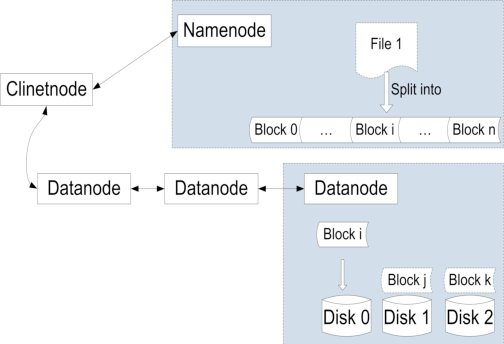
\includegraphics{figure1}
	\caption{HDFS Architecture Block N represents $N_{th}$ file block of File ``1'' on HDFS}
	\label{figure1}
\end{figure}

Blocks of files are distributed in the two-tiered storage achitechture, Datanode and Datanode's disk. It will make full use of the
collective bandwidth of HDFS if each replica of blocks is appropriately choosen and scheduled to reduce remoting reading among
Datanodes. \par
MapReduce is usually introduced as a computation model cooperating with HDFS. It can process the data with good locality.
However, due to the traits of scientific data and the operation pattern, MapReduce cannot be directly utilized on scientific-data
analysis with perfect performance.

\subsection{Scientific-data Analysis}
Scientific-data are usually stored in high-structured files, a kinds of spectial binary format, which can not be read directly by
MapReduce. Each file contain multi logical units, and each unit are corresponding to its own phsical meaning. The size of 
each logical varies a lot in one file and only same logical units can be manipulated in most of analysis operations. \par
In this paper, climte model data is used, the total size of which is extremely huge. One single file of CAM at 0.125 degrees,
an atmosphere model from NCAR\cite{neale2010description}, is 24GB size along with one single 3D variable is 616MB and one 2D variable 
is 24MB. It is 28.8TB size of 100 years of monthly output\cite{jacob2012new}. These data are organized by thousands of files with 
timestamp named in NetCDF format, called history result. Each file contains the same dozens of physical variables. Analysis 
operations need to process the whole or part of the history results. These operations include computing average, combining the same 
variables in different files, producing the remapping file and fast fourier transform (FFT), etc. They require to handle whole or
part of variables in multi-files.

\subsection{Problems and Chanllenges} 
Problem/Challenge 1: How to define the operation unit considering the storage unit? Logical unit size varies a lot from a few bytes to
gigabytes. Then it can not be used as the operation unit. Otherwise, the workflow of each task will be imbalance. \par
Problem/Challenge 2: How to schedule tasks among many files to increases the locality and reduce the data network transfer? If all logical
units with same meanings locate on the same Datanode, all data access will proceed locally. However, default block placement policy of HDFS
cannot ensure that, which leads huge amount data network transfer, as the above mentioned. \par
Problem/Challenge 3: How to best utilize the disk I/O? There may be multi disks in one Datanode. It can not take use of disks thoughput if
reading operations is serial or processing, reading and transferring is non-overlapping.  

\section{Parallel scientific-data analysis}
In order to solve the problems mentioned in previous section to take full use of distributed I/O performance, we propose a new framework 
--- Parallel Scientific-data Analysis (ParSA). 

\subsection{Logical Unit Split and Group among File Blocks}
No matter how a file is split, all data in one block are stored contiguously in a physical location, since file block is the storage
unit of HDFS. Thus the block of HDFS can be used as the basic operation unit to keep continuity in disk and improve I/O performance 
by proper scheduling to reduce network read. In a block, we can group the small size of logical units or split the big size one.\par
The logical unit split and group approach is shown in Figure.\ref{figure2}. All logical units located in one block are distributed 
into one group. If a logical unit spans two or more blocks, this logical unit will split to several parts. For example, LU1 spans three 
blocks. It will split into three split parts - LU1 (1), LU1 (2) and LU1 (3), unique identifier assigned to each part. Then LU1 (1) 
and LU0 locate in file block 0 and form a operation unit group. LU1 (2) itself is distributed as a group. The remaining LU1 (3), LU2 
and LU3 are distributed to the third group. The mapping relationship between groups and file blocks should be records, as shown in 
Figure.\ref{figure3}. \par

\begin{figure}
	\centering
	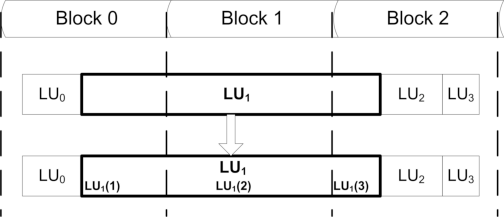
\includegraphics{figure2}
	\caption{Logical Units Spliting and Grouping into HDFS Block. $LU_N$ presents $N_{th}$ logical unit. $LU_N(i)$ stands for 
			$i_{th}$ part of $LU_N$}
	\label{figure2}
\end{figure}

\begin{figure}
	\centering
	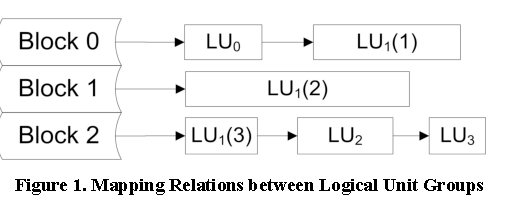
\includegraphics{figure3}
	\caption{Mapping Relationship between Logical Unit Groups and File Blocks}
	\label{figure3}
\end{figure}

Variables in NetCDF, used in climate data, can be viewed as multi-dimension array. An array section is defined as a contiguous rectangular
block specified by two vectors - index vector and count vector. The index vector indicates the start offset of the element in the corner
closest to the orign. The count vector gives the lengths of the edges along each of the variable's dimension. \par
For instance, the variable given in Figure.\ref{figure4a} is a two-dimension slab. If we access the whole variable, index vector is (0, 0) 
and count vector is (3, 5). However, if this variable locates on two file blocks stored with HDFS, and variable are split between value 
(1, 1) and value (1, 2), it cannot be split into these two pieces. The reason is that each of part is not a rectangular shape, which 
can not use an index vector and count vector to represent. In this situation, we should split the variable into four pieces, as 
Figure.\ref{figure4b} shows.

\begin{figure}[htb]
    \centering
    \begin{subfigure}{.5\textwidth}
        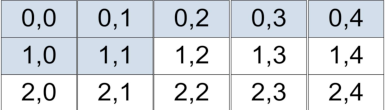
\includegraphics[width=\textwidth]{figure4a}
        \caption{}
        \label{figure4a}
    \end{subfigure}

    \begin{subfigure}{\textwidth}
        \centering
        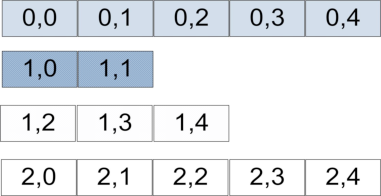
\includegraphics[width=.5\textwidth]{figure4b}%
        \caption{}
        \label{figure4b}
    \end{subfigure}
    \caption{Variable Split in NetCDF. (a) Variable to be split. (b) The split result of variable given in (a). The index vectors of four
            split slab are (0, 0), (1, 0), (1, 2) and (2, 0) respectively. And the counts vectors are (1, 5), (1, 2), (1, 3) and (1, 5) 
            respectively.}
\end{figure}

\subsection{Scheduler}
As discussed in section 2.3, quite a few operations are only executed on the same logical units among multi-files. In principle, blocks 
containing these units should be scheduled in one Datanode as many as possible to increase the acess locality. \par
At first, information about file distribution should be gathered. As discussion in section 2.1, file block has three replicas by default. 
In this paper, we define the tuple (Ni, Dj) as the location of a file block, which means Datanode number and hard disk number, respectively. 
Assume we get the following block location information for the first file block of all three files. \par

$$\begin{array} {lcrr}
F0,B0: & (N0,D0) & (N1,D2) & (N5,D1) \\
F1,B0: & (N0,D1) & (N2,D0) & (N3,D1) \\
F2,B0: & (N1,D2) & (N6,D0) & (N7,D1)
\end{array}$$

For the nine replicas for B0 of F1, F2 and F3, Datanode N0 covers 2 replicas. N1 contains 2 replicas and other Datanode only contain 1 for 
each. Then Datnode N0 and N1 contain the same number of replicas. Therefore, Datanode N0 is chosen to process the B0 block of F1 and F2,
instead of N1 to process B0 of F0 and F2. The reason is that B0 of F0 and F2 locates on the same hard disk in N1 Datanode, which is more 
likely to impact the performance (explained in section 3.3). Although N1, N6 and N7 all have the B0 relica of F2, N1 is selected. 
Because when disk 0 of N0 is broken, the relica B0 of F0 can be accessed in N1. Accroding to this principle, other blocks can be scheduled
as the Figure.\ref{figure5b} shown.

\begin{figure}[htb]
    \centering
    \begin{subfigure}{.5\textwidth}
        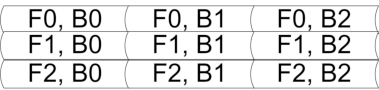
\includegraphics[width=\textwidth]{figure5a}
        \caption{}
        \label{figure5a}
    \end{subfigure}

    \begin{subfigure}{.5\textwidth}
        \centering
        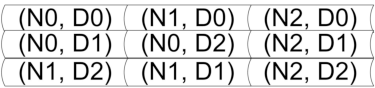
\includegraphics[width=\textwidth]{figure5b}%
        \caption{}
        \label{figure5b}
    \end{subfigure}
    \caption{Task Scheduler of ParSA. (a) Three files stored in HDFS. (b) Static task scheduler result of ParSA for the three files in (a). FN presents the $N_{th}$ file to be processed; BN presents $N_{th}$ file block on HDFS; (Ni, Dj) stands for corresponding file block 
    in (a) locates on $j_{th}$ disk of $i_{th}$ Datanode.}
    \label{figure5}
\end{figure}

\subsection{Workflow of ParSA}
Although we utilize the file block location in HDFS to schedule which block replica are selected among Datanodes, I/O bandwidth of disks may 
not be efficiently utilized intra-Datanode. For example, the file block B0s of F0 and F1 are assigned to N0 in Figure.\ref{figure5}. Even
though B0 of F0 and B0 of F1 locate on different disks - D0 and D1 respectively, the two disks are accessed sequentially instead of 
parallelly, if the operations are implement from logical level at Datanode N0 as following:

\begin{algorithm}[htb]
\caption{Sequential operation on disk in the same Datanode} 
\label{alg:sequential-operation}
\begin{algorithmic}
\FOR{each logical-unit \textbf{LU} in B0}
\FOR{each file \textbf{Fx} whose block B0 locates on N0}
\STATE read \textbf{LU} from B0 of Fx
\STATE operate on \textbf{LU} 
\ENDFOR
\ENDFOR
\end{algorithmic}
\end{algorithm}

In this paper, we propose a new workflow to efficiently access the data on HDFS and maximize utilizing all disk bandwidth in one 
Datanode. \par
In ParSA, the framework of hybird of MPI and pthread is used. MPI is responsible for parallelism and communication among Datanodes. There
is one MPI process in each Datanode. Pthead is responsible to implement the detail operations within each Datanode, constituting of 
three major components: reading-thread, processing-thread and receiving-thread. \par
\textbf{Reading-thread} If more than one thread dedicatedly access one disk, it cannot get a higher performance than only one thread. 
Thus we invoke one thread for each disk. This is defined as reading-thread and use $Tread_i$ to present the $i_{th}$ reading-thread. 
For each block, $Tread_i$ reads the queue of logical units, shown in Figure.\ref{figure3}. After reading the logical unit, it is 
marked as LOCAL\_FLAG, distinguishing with receiving data. The workflow of reading-thread is given below:

\begin{algorithm}[htb]
\caption{reading-thread} 
\label{alg:reading-thread}
\begin{algorithmic}
\STATE inputs:
\STATE \textbf{datanode\_number}:the Datanode where the reading-thread locates.
\STATE \textbf{disk\_number}:the disk number to be accessed. 
\STATE \textbf{scheduler\_result}:task scheduler result, given in Figure 5(b).
\STATE \textbf{LU\_groups\_map}:mapping relations between logical unit groups and file blocks in Figure 3.
\newline
\FOR{each tuple (node\_no, disk\_no) in \textbf{scheduler\_result}} 
\IF{node\_no = \textbf{datanode\_number} and disk\_no = \textbf{disk\_number}}
\STATE get the \textbf{file-index} and \textbf{block-index} according to the index of tuple, shown in Figure 5(a).
\FOR{each \textbf{lu} in \textbf{LU\_groups\_map[block\_index]}}
\STATE read \textbf{values} of \textbf{lu} of \textbf{file\_index} file
\STATE store \textbf{file-index} and \textbf{values} into \textbf{lu}
\STATE mark \textbf{lu} as \textbf{LOCAL\_TAG}
\STATE insert (\textbf{lu}) into data queue
\STATE notify processing-thread
\ENDFOR
\ENDIF
\ENDFOR
\STATE send \textbf{ending-flag} to processing-thread
\end{algorithmic}
\end{algorithm}

\textbf{Processing-thread} After reading-threads read logical units into queue, the processing-thread will be waked up. The processing-
thread takes in charge of calling user-defined function local\_data\_process to process these logical units. Users only focus on 
implementing operations on logical unit. Since each Datanode only covers part of entire dataset, the major process should reduce the 
intermediate results, computed with each process in each Datanode. This operation is another user-defined recv\_data\_process function. 

\begin{algorithm}[htb]
\caption{processing-thread} 
\label{alg:processing-thread}
\begin{algorithmic}
\STATE inputs:
\STATE \textbf{num\_tasks}:total number of \textbf{ending-flag} to wait
\STATE \textbf{intermediate\_results}:store the intermediate results
\newline
\STATE \textbf{cur\_num\_tasks} = 0
\WHILE{$\textbf{cur\_num\_tasks} < \textbf{num\_tasks}$}
\STATE wait until receiving notification
\IF{receive \textbf{ending-flag}}
\STATE $\textbf{cur\_num\_tasks++}$
\STATE fetch the logical unit queue
\FOR{each \textbf{lu} in logical unit queue}
\STATE get \textbf{interm\_res} according to \textbf{lu identifier} 
\IF{\textbf{lu's} flag == LOCAL\_FLAG}
\STATE call \textbf{local\_data\_process} (\textbf{lu}, \textbf{interm\_res})
\ENDIF
\IF{\textbf{lu's} flag == RECV\_FLAG}
\STATE call \textbf{recv\_data\_process} (\textbf{lu}, \textbf{interm\_res}) 
\ENDIF
\IF{is not major process}
\IF{all logical unit are processed in this Datanode}
\STATE store \textbf{interm\_res} into lu
\STATE mark lu as \textbf{RECV\_TAG}
\STATE send (lu) to major process
\ENDIF
\ENDIF
\ENDFOR
\ENDIF
\ENDWHILE
\end{algorithmic}
\end{algorithm}

\textbf{Receiving-thread} Receiving-thread is a component in major process. It receives logical inits from worker processes, and
puts the logicl units into the receiving queue. Then the processing-thread is notified to fetch these data. \par
The workflow of ParSA is shown in Figure.\ref{figure6}. Major process locates in Datanode 0, and a worker process is presented as 
Datanode 2. Each reading thread reads the logical units which is assigned to this thread. After $Tread_0$ in Datanode 2 reading the 
logical LU1(3) of F0, it reads LU2 of F0, inserts the values into queue and notifies processing-thread to wake up. The processing-thread 
processes all the values in queue sequentially. When processing-thread detects that LU1(3) are all processed in Datanode 2, it will 
send the intermediate results to the major process. Once Receiving-thread in major process gets the intermediate results, it inserts the results into the logical unit queue. Since the logical unit queue is the shared resource, all threads must access exclusively. \par

\begin{figure}[htb]
    \centering
    \begin{subfigure}{1\textwidth}
        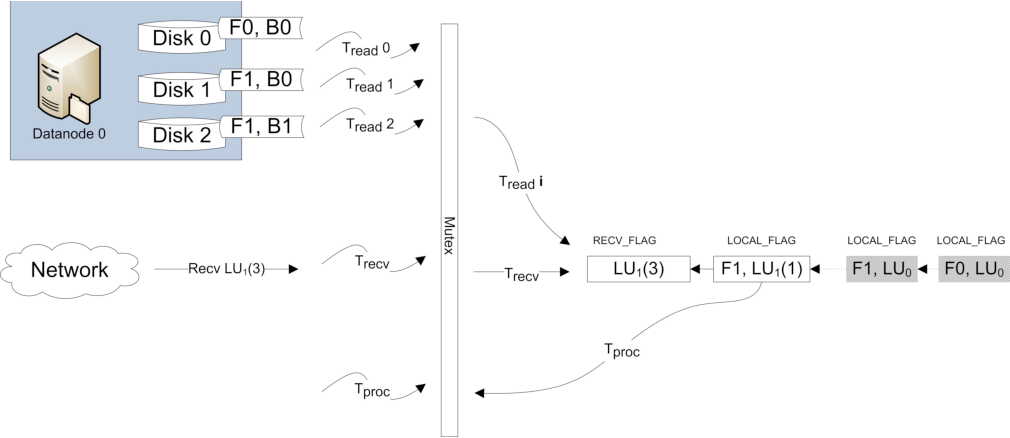
\includegraphics[width=\textwidth]{figure6a}
        \caption{}
        \label{figure6a}
    \end{subfigure}

    \begin{subfigure}{\textwidth}
        \centering
        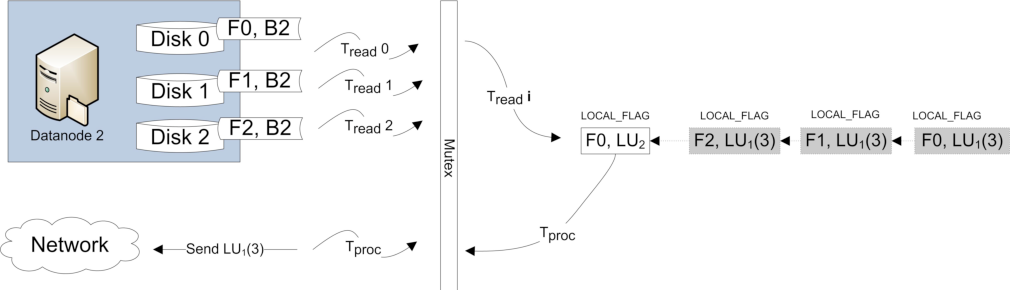
\includegraphics[width=1\textwidth]{figure6b}%
        \caption{}
        \label{figure6b}
    \end{subfigure}
    \caption{Workflow of ParSA. (a) Major process; (b) Worker process. The logical units with gray background stand for already-processed
             logical unit.}
    \label{figure6}
\end{figure}


ParSA is the framework for scientific-data access on HDFS. Users can only put their focus on logical operations. ParSA is implemented 
using MPI and Pthread, providing more flexible configration with regard to performance than MapReduce. ParSA can achieve load-balance based
on current block replicas layout information. However, if the layout itself is unbalanced, the performance is also impacted. In the next 
section, how to further improve the performance by optimizing layout will be discussed.

\section{Block layout optimization}
In section 3.2, the scheduler of ParSA utilizes the location information of file blocks. In principle, file blocks containing the same
logical units in the one Datanode should be scheduled as many as possible for the operations involving multi-files, while the default
block layout strategy of HDFS cannot guarantee this. \par
In HDFS, if Clientnode is one of the Datanodes, the first replica of each file block will be stored in Clinenode, and other replicas are 
chosen random Datanodes expect for Clientnode. If the Clientnode is not Datanode, the fisrt replica will be randomly stored in a 
Datanode. \par
Although the scheduler can assign tasks based on current file block replicas distribution, the distribution should be control according 
to the principle for task assignment in order to achieve load balancing. Since blocks of files are stored in Datanode and Datanode's disk,
it needs to optimize the layout in these the two tiered architecture. 

\subsection{Data layout inter-Datanodes}
Taken into account the characteristic of scientific-data analysis, tightly coupled data as above described should be assigned in one 
Datanode to increase locality of processing data. Simultaneously, each Datanode should have equal workload, with a pretty load-balance 
performance. \par 
However, it may indeed exits a few analysis operations different from the characteristic. ParSA expose an interface for users to determine
where the first replicas of blocks should locate. What's more, the second replicas are stored with uniform distribution automaticlly.
The third abide by the HDFS default strategy.  

\subsection{Data layout intra-Datanodes}
As discussed in section 3.3, the workflow of ParSA invokes one thread for one disk. If blocks are imbalance among disks in one Datanode, 
it will waste the bandwidth of other disks. The load balance is not only the equal number of file blocks per disk in one Datanode, but 
also the distribution of blocks containing the same logical units. The former can be guaranteed by HDFS default disk allocation strategy
with a round-robin way, while the later can not be satisfied all the time. ParSA provides a round-robin mechanism for these blocks 
distribution, as shown in Figure.\ref{figure7}. The disk will be used for a block, if it does not store one with the same logical 
units. \par

\begin{figure}[htb]
    \centering
    \begin{subfigure}{0.5\textwidth}
        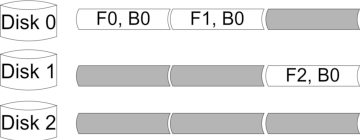
\includegraphics[width=\textwidth]{figure7a}
        \caption{}
        \label{figure7a}
    \end{subfigure}

    \begin{subfigure}{\textwidth}
        \centering
        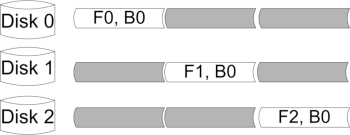
\includegraphics[width=0.5\textwidth]{figure7b}%
        \caption{}
        \label{figure7b}
    \end{subfigure}
    \caption{Round-robin Method for File Block with Same Meaning. (a) Block layout unbalance for B0. There are two B0s locate on Disk 0
             while Disk 2 contains no B0. (b) Using the improved strategy. B0s are stored in a round-robin way and locate evenly among 
             disks.}
    \label{figure7}
\end{figure}

\section{Evalution}

\subsection{Experimental setting}
To demonstrate the performance portability of ParSA framework, we choose two HDFS clusters with different configuration, as shown in Table
.\ref{table1} and Table.\ref{table2}. \par

\begin{table}[ht]
\caption{System Configuration of hadoop cluster 1} 
\centering 
\begin{tabular}{c c}
\hline
configuration & parameter \\
\hline 
\#nodes & 16 \\ 
\#disks per node & 2x1 TB SATA2 \\
OS & RedHat 6.2 \\
MPI & Intel® MPI Library 3.2 \\
Compiler & Intel® Composer XE 2011 \\
NetWork & Infiniband QDR \\
CPU & Intel® Xeon® Processor E5620 @2.4GHz \\
Memory & 48GB \\
Hadoop & Apache Hadoop 1.0.3 \\
\hline 
\end{tabular}
\label{table1} 
\end{table}

\begin{table}[ht]
\caption{System Configuration of hadoop cluster 2} 
\centering 
\begin{tabular}{c c}
\hline
configuration & parameter \\
\hline 
\#nodes & 6 \\ 
\#disks per node & 5x500 GB SAS \\
OS & RedHat 6.2 \\
MPI & Intel® MPI Library 4.1 \\
Compiler & Intel® Composer XE 2011 \\
NetWork & Dual GigE Ethernet \\
CPU & Intel® Xeon® Processor E5645 @2.4GHz \\
Memory & 48GB \\
Hadoop & Apache Hadoop 1.0.3 \\
\hline 
\end{tabular}
\label{table2} 
\end{table}

In order to demonstrate the efficiency of ParSA, we use climate data generated by a ocean model, POP, a component of climate model. The 
dataset has 100 NetCDF files, and each of file contains 60 two-dimension variables (logical units) and 18 three-dimension variables, with
320x384 and 320x384x40 resolution, which has 309 MB datasize. The total size of this dataset is 30.9 GB. \par 
The major analysis operation is calculating time average using ncea command of NCO package, which is the basic preprocessing operation
for almost all of climate data analysis. \par
To evaluate the scalability of ParSA, we compare the speedup and throughput performance of different number of Datanodes and different
number of disks per node. Cluster 1 is used for the former experiment since the number nodes is more than cluster 2. While 
cluser 2 is used for the later experiment since each node has more disks in cluster 1. \par 

\subsection{Scalability with different disks per Datanode}
ParSA can get about 1.3 GB/s aggregation throuphout if per Datanode uses 5 disks, as shown Figure.\ref{figure8a}. The throughput has a 
remarkable scalability if per Datanode uses 1 to 4 disks. However, it has little performance improvement with 5 disks. The reason is 
that there are some serial operations, such as writing results and communication, which impact on the performance. Since a series of 
strategies propused by ParSA is aimed at I/O, Figure.\ref{figure8b} shows the speedup with only reading part. It's scalability is close
to the ideal speedup. 

\begin{figure}[tbh]
    \centering
    \begin{subfigure}{0.5\textwidth}
        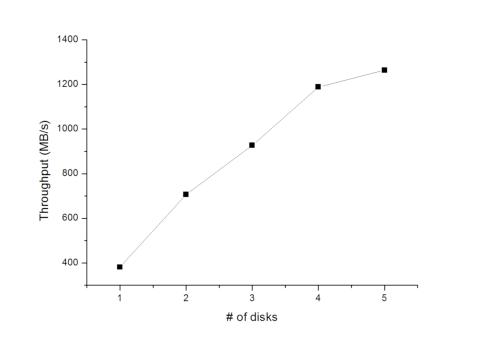
\includegraphics[width=\textwidth]{figure8a}
        \caption{}
        \label{figure8a}
    \end{subfigure}\begin{subfigure}{0.5\textwidth}
        \centering
        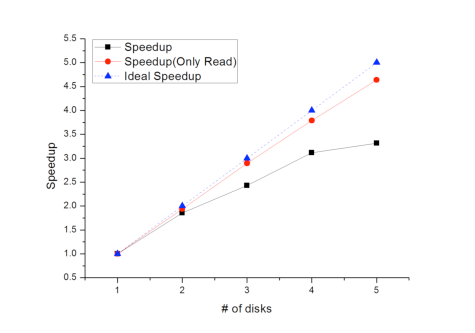
\includegraphics[width=\textwidth]{figure8b}%
        \caption{}
        \label{figure8b}
    \end{subfigure}
    \caption{Scalability of ParSA along with different number of disks per Datanode. (a) Throughput; (b) Speedup.}
    \label{figure8}
\end{figure}

\subsection{Scalability with different Datanodes}
Two disks per node are used in this evaluation with cluster 1. It almost keeps the linear speedup until 9 Datanodes as shown Figure 9. 
However, the performance improvment is limited when the Datanodes are greater than 9 due to the increasing overhead of communication
and the critical section controlled by mutex, as shown Figure.\ref{figure6}. Although data processing is overlapped with data accessing, 
the time non-overlapped occupies almost 38.89\% on 16 datanodes, and this proportions are only 0.02\% and 7.96\% when datanodes are 9 
and 12 respectively. \par
In Figure.\ref{figure9a}, it can get about 800MB/s maximum throughput on 12 datanodes, with 24 disks totally. While the same number of 
disks in Figure.\ref{figure8a}, 4 disks per datanode, it can get about 1.2GB/s. The same performance only need 2 disks per datanode, 
with 12 disks totally. The reason is that, on one hand, the disks and network are difference between the two cluters; on the other hand,
cluster 1 requires more network access due to the few disks per node.  \par
The speedup of only reading is presented as Figure.\ref{figure9b}, which shows an exllcent scalability with different datanodes. The 
reason why the speedup is higher than the ideal may result from performance variability. 

\begin{figure}[tbh]
    \centering
    \begin{subfigure}{0.5\textwidth}
        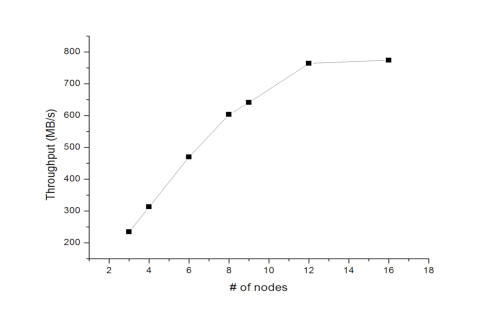
\includegraphics[width=\textwidth]{figure9a}
        \caption{}
        \label{figure9a}
    \end{subfigure}\begin{subfigure}{0.5\textwidth}
        \centering
        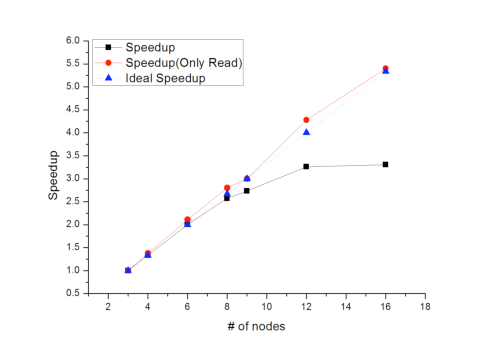
\includegraphics[width=\textwidth]{figure9b}%
        \caption{}
        \label{figure9b}
    \end{subfigure}
    \caption{Scalability of ParSA along with different number of Datanodes. (a) Throughput; (b) Speedup.}
    \label{figure9}
\end{figure}

\subsection{Throughput comparision with different task optimization strategies}
HDFS block is the basic operation unit in ParSA, spliting and grouping the logical unit. We select the block replicas in different 
Datanodes to reduce network reading, optimize the workflow to support overlapping and parallelism of reading and processing, as well as 
the optimization of blocks layout for both inter-datanodes and intra-datanodes. \par
To present the improving performance, two additional strategies are compared to ParSA. The first one takes logical unit as the operation
unit. The disk utilization is shown as Figure.\ref{figure10a}. Since the size of logical unit varies quite a lot, a serious load imbalance
exists among tasks. The second strategy takes all logical units located in one file block as an operation unit, while those logical unit 
which locate on more than one block do not be split and treat the big size logical units as other operation unit. In this situation, it can
not guarantee that an entire operation unit stores in a disk. When a thread try to read this unit, it requires read a part of value from the
other disk. In the mean time, the other thread is reading the same disk, leading to disk resource competition. This utilization performance
is presented as Figure.\ref{figure10b}. \par
Compared with throuphput to evaluate the speedup, ParSA outperforms the above two strategies by a factor of 3.34X and 1.14X respectively.

\begin{figure}[tbh]
    \centering
    \begin{subfigure}{0.5\textwidth}
        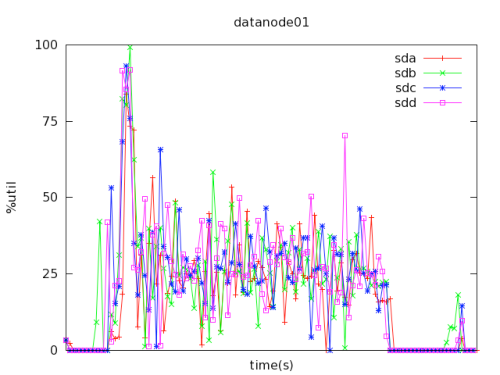
\includegraphics[width=\textwidth]{figure10a}
        \caption{}
        \label{figure10a}
    \end{subfigure}\begin{subfigure}{0.5\textwidth}
        \centering
        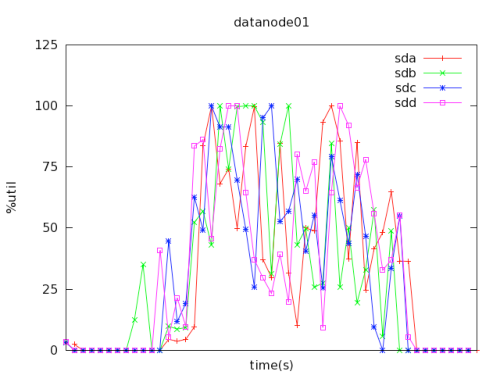
\includegraphics[width=\textwidth]{figure10b}%
        \caption{}
        \label{figure10b}
    \end{subfigure}
    \begin{subfigure}{0.5\textwidth}
        \centering
        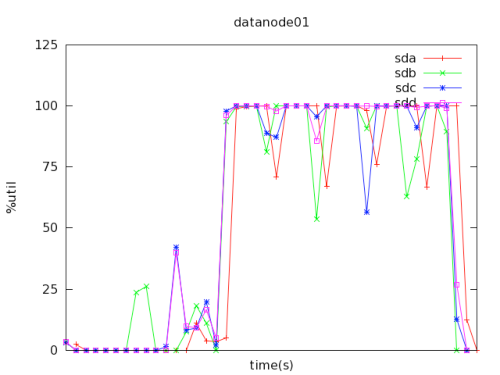
\includegraphics[width=\textwidth]{figure10c}%
        \caption{}
        \label{figure10c}
    \end{subfigure}
    \caption{Comparison of Disk-utilization with Different Task Assignment Strategies. (a) Logicl Unit. (b) Block Unit without Splitting. 
             (c) Strategy of ParSA}
    \label{figure10}
\end{figure}

\section{Conclusion and future work}
A high-throughput and scalable scientific framework combined with HDFS distributed file system and NCO analysis tool has been designed, 
implemented and evaluated. Maximize distributed I/O performance has been gained by scheduling block repicas in different datanodes, 
optimizing the blocks layout for both inter-datanodes and intra-datanodes,  as well as overlapping the data reading, processing and 
transferring. Instead of Hadoop framework, we use multi-process with MPI to parallel the NCO basic operations, without leading to compatible 
problem. In future work, we plan on testing the framework on some complex climate data analysis, such as FFT, principal component analysis 
and Wavelet transform.

%\label{text}
	
%% The Appendices part is started with the command \appendix;
%% appendix sections are then done as normal sections
%% \appendix

%% \section{}
%% \label{}

%% If you have bibdatabase file and want bibtex to generate the
%% bibitems, please use
%%
\bibliographystyle{elsarticle-num} 
\bibliography{zhangtao}

%% else use the following coding to input the bibitems directly in the
%% TeX file.

%\begin{thebibliography}{00}

%\bibitem{label}
%% Text of bibliographic item

%\bibitem{text}

%\end{thebibliography}

\end{document}
\endinput
%%
%% End of file `elsarticle-template-num.tex'.
